
\chapter{Algebra und Gleichungen}
\label{chap:III_algebra}
\label{chap:III_qubit}
\setcounter{section}{3}
\setcounter{subsection}{0}
\setcounter{subsubsection}{1}
\setcounter{secnumdepth}{3}
\subsection{Die arabische Mathematik und die Geburt der Algebra}
\label{sec:3.1_arabische_mathematik}

Nach den Griechen, Indern und Babyloniern war es die arabisch-islamische Welt, 
die die Mathematik auf eine neue, systematische Ebene hob. 
Während in Europa das antike Wissen weitgehend verloren ging, 
bewahrten und erweiterten Gelehrte wie 
\emph{al-Chwarizmi}\index{al-Chwarizmi, Muhammad ibn Musa}, 
\emph{Omar Chayyām}\index{Chayyām, Omar} und 
\emph{al-Karaji}\index{al-Karaji, Abu Bakr} die Erkenntnisse ihrer Vorgänger. 

Im 9.~Jahrhundert verfasste \emph{al-Chwarizmi} in Bagdad das Werk 
\emph{„Kitāb al-jabr wa’l-muqābala“}\index{Kitāb al-jabr wa’l-muqābala}, 
das als Geburtsstunde der \emph{Algebra}\index{Algebra} gilt. 
Der Begriff „al-jabr“ bedeutet sinngemäß „das Wiederherstellen“ oder „das Ergänzen“, 
„al-muqabala“ bezeichnet „das Gegenüberstellen“. 
Gemeint war damit eine Methode, Unbekanntes zu isolieren und Gleichungen zu vereinfachen – 
eine Revolution im Denken über Zahlen und Formen. 

\HistoryBox{Von der Praxis zur Theorie}{hist:algebra_praxis}{
	Im Mittelpunkt der arabischen Mathematik stand anfangs die Lösung praktischer Probleme: 
	Verteilung von Erbschaften, Berechnung von Grundstücksflächen, 
	Bestimmung von Handelsanteilen oder astronomische Messungen. 
	Doch aus diesen konkreten Aufgaben entwickelte sich ein allgemeines Verfahren, 
	Unbekannte zu bestimmen – die Geburt der symbolischen Methode.
}

Ein klassisches Beispiel aus der frühen arabischen Mathematik ist die Berechnung von Erbanteilen. 
Nach islamischem Recht erhält eine Frau den achten Teil des Nachlasses, 
der Rest wird unter den Söhnen gleich verteilt. 
Beträgt das Erbe insgesamt 600~Dinar, so ergibt sich:

\[
1 = \tfrac{1}{8} + 2x,
\]
wobei \(x\) den Anteil eines Sohnes beschreibt. 
Nach Umformen folgt \(x = \tfrac{7}{16}\). 
Damit erhält jeder Sohn \(x \cdot 600 = 262{,}5\)~Dinar, 
die Frau \(75\)~Dinar.

\DidaktikBox{Vom praktischen Problem zur abstrakten Gleichung}{did:algebraischer_denken}{
	Die arabischen Mathematiker formulierten solche Beziehungen symbolisch 
	und lösten sie durch \emph{al-jabr} (Ergänzen) und \emph{al-muqabala} (Gegenüberstellen). 
	So entstand aus einem alltäglichen Rechenproblem die Idee der allgemeinen Gleichung – 
	der Beginn der Algebra als abstraktes Denken.
}

\HinweisBox{Ein gemeinsames Erbe}{hinweis:algebra_herkunft}{
	Die arabischen Mathematiker erfanden die Algebra nicht aus dem Nichts. 
	Sie knüpften an das Wissen der Babylonier, Griechen und Inder an. 
	Schon die Babylonier lösten Gleichungen der Form \(x^2 + bx = c\) 
	mit tabellarischen Methoden, und die Griechen beschrieben geometrische Zusammenhänge, 
	die im Kern algebraisch waren. 
	In Indien entstanden symbolische Rechenverfahren für Unbekannte (\emph{yāvattavat}). 
	Die arabischen Gelehrten verbanden all diese Traditionen, 
	gaben ihnen eine einheitliche Sprache und machten daraus ein geschlossenes System – 
	die \emph{Al-jabr}, die wir heute Algebra nennen.
}

Ein bekanntes Beispiel aus Al-Chwarizmis Werk lautet:
\begin{quote}
	„Ein Quadrat und zehn seiner Wurzeln ergeben neununddreißig.“
\end{quote}
Heute würden wir dies als
\[
x^2 + 10x = 39
\]
schreiben.  
Al-Chwarizmi dachte jedoch geometrisch: Das Glied \(x^2\) stellte ein Quadrat dar, 
dessen Seitenlänge \(x\) ist. Die Terme \(10x\) bildeten zwei Rechtecke der Breite~5, 
die an zwei Seiten des Quadrats anliegen.  
Das fehlende kleine Quadrat in der Ecke, das die Figur zu einem größeren Quadrat ergänzt, 
hat die Fläche \(5^2 = 25\).  
Durch Hinzufügen dieser Fläche wird das Gebilde zu einem vollständigen Quadrat:
\[
x^2 + 10x + 25 = 39 + 25,
\]
also \((x+5)^2 = 64\), woraus \(x = 3\) folgt.
\subsubsection*{Graphische Darstellung der quadratischen Ergänzung}
\phantomsection
\begin{figure}[h!]
	\centering
	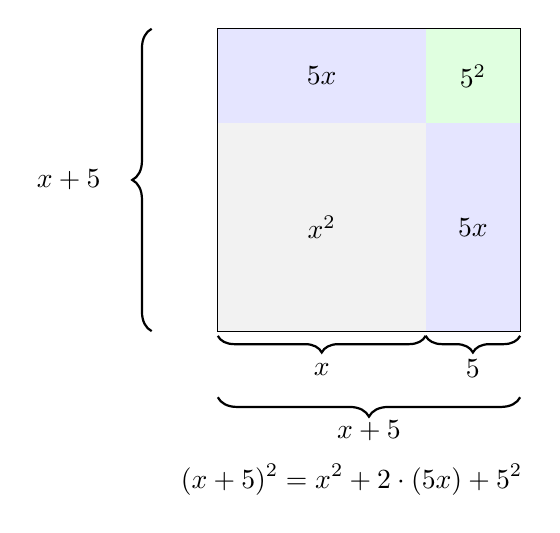
\begin{tikzpicture}[scale=0.12, thick]
		\def\xlen{22}   % Länge x (grafisch)
		\def\five{10}   % Länge 5  (grafisch)
		
		% Gesamtquadrat (x+5)
		\draw (0,0) rectangle (\xlen+\five,\xlen+\five);
		
		% Unterteilung
		\draw (\xlen,0) -- (\xlen,\xlen+\five);
		\draw (0,\xlen) -- (\xlen+\five,\xlen);
		
		% Füllungen
		\fill[gray!10] (0,0) rectangle (\xlen,\xlen);                 % x^2
		\fill[blue!10] (0,\xlen) rectangle (\xlen,\xlen+\five);       % 5x (oben)
		\fill[blue!10] (\xlen,0) rectangle (\xlen+\five,\xlen);       % 5x (rechts)
		\fill[green!12] (\xlen,\xlen) rectangle (\xlen+\five,\xlen+\five); % 5^2
		
		% Beschriftungen
		\node at ({\xlen/2},{\xlen/2}) {$x^2$};
		\node at ({\xlen/2},{\xlen+\five/2}) {$5x$};
		\node at ({\xlen+\five/2},{\xlen/2}) {$5x$};
		\node at ({\xlen+\five/2},{\xlen+\five/2}) {$5^2$};
		
		% Nur eine geschweifte Klammer unten (5 dann x)
	%	\draw [decorate, decoration={brace, amplitude=6pt}]
	%	(0,-2) -- (\five,-2) node[midway, yshift=-10pt] {$5$};
		\draw [decorate, decoration={brace, amplitude=6pt,mirror}]
		(0,-0.5) -- (\xlen,-0.5) node[midway, yshift=-12pt] {$x$};
			\draw [decorate, decoration={brace, amplitude=6pt,mirror}]
		(\xlen,-0.5) -- (\xlen+10,-0.5) node[midway, yshift=-12pt] {$5$};
		% Gesamtlänge unten (x+5)
		\draw [decorate, decoration={brace, amplitude=7pt,mirror}]
		(0,-7) -- (\xlen+\five,-7) node[midway, yshift=-12pt] {$x+5$};
		
		% Linke Gesamtlänge (optional, schmal)
		\draw [decorate, decoration={brace, amplitude=7pt}]
		(-7,0) -- (-7,\xlen+\five) node[midway, xshift=-30pt] {$x+5$};
		
		% Titel
		\node[below right] at (-5,\xlen+\five-45)
		{$\displaystyle (x+5)^2 = x^2 + 2\cdot(5x) + 5^2$};
	\end{tikzpicture}
	\caption{Aus den Teilflächen $x^2$, $5x$ und $5^2$ entsteht das Quadrat $(x+5)^2$.}
\end{figure}





Diese geometrische Methode des Ergänzens – das eigentliche „al-jabr“ – 
führte direkt zur allgemeinen Regel für quadratische Gleichungen, 
die wir heute in symbolischer Form schreiben.  

\DidaktikBox{Der Ursprung des Wortes „Algorithmus“}{did:algorithmus}{
	Der Name \emph{al-Chwarizmi} wurde im Lateinischen zu „Algoritmi“ verfremdet. 
	Daraus entstand das Wort \emph{Algorithmus}\index{Algorithmus}. 
	Damit geht auch ein zweiter Grundpfeiler der modernen Mathematik 
	– die systematische, regelhafte Berechnung – 
	auf die arabische Wissenschaft zurück.
}

Die Algebra war also weniger eine Entdeckung im modernen Sinn, 
sondern eine geistige Neuordnung des vorhandenen Wissens. 
Sie verband die indischen Zahlensysteme mit griechischer Geometrie 
und formte daraus ein allgemeines Rechenverfahren. 
Damit begann die Mathematik, ihre eigene Sprache zu entwickeln – 
eine Sprache der Symbole, Regeln und Abstraktionen.

\subsection{Gleichungen als Werkzeuge zur Problemlösung}
Gleichungen wurden zum universellen Werkzeug, um unbekannte Größen zu berechnen. 
Von einfachen linearen Gleichungen bis zu quadratischen Formen zeigte sich ihre enorme Nützlichkeit. 

\subsection{Die Entstehung der komplexen Zahlen}
Bei der Lösung höherer Gleichungen traten scheinbar „unmögliche“ Zahlen auf. 
Aus dieser Notwendigkeit heraus entstanden die komplexen Zahlen, die bald eine tiefe Bedeutung erhielten. 

\subsection{Mathematik als System von Regeln}
Mit Algebra und Gleichungen begann die Mathematik, sich stärker als ein in sich geschlossenes Regelwerk zu verstehen. 
Diese Sichtweise prägte die weitere Entwicklung bis in die Moderne. 
